\section{Introduction}
\begin{spacing}{2}
    \par
    Driven by escalating competition in traditional educational settings, the prevalence of supplementary tutoring beyond the standard school schedule has surged, becoming a prevalent tactic for students striving to secure an advantageous position in scholastic endeavors. It is extensively acknowledged that students hailing from lower socioeconomic status (SES) families tend to underperform academically compared to their higher-SES counterparts. \citep{zhou2015family}.  
    
    \par
    Show your research objectives by bulleted or numbered list. 
    
    \begin{enumerate}
        \item This is my first point. 
        \item This is my second point. 
        \item And my third research objective. 
    \end{enumerate}
    
    \par
    
    \subsection{Table}    
    \par
    Talk is cheap, now show me the data! 
    
    \begin{table}[h]
    	\caption{A Table Demo}
    	\begin{tabular}{l c c c c}
    		\toprule
    		Column 0 & Column 1 & Column 2 &  Column 3 & Column 4 \\
    		\midrule
    		Row 0 		& 1 & 12.05 & 4.60\% & 71.68 \\
    		Row 1 		& 117 & 81.88 & 96.58\% & 1.71 \\
    		Row 2 		& 15 & 84.93 & 100\% & 0.00 \\
    		Row 3 		& 343 & 61.49 & 61.81\% & 20.12 \\
    		Row 4 		& 242 & 73.92 & 94.21\% & 0.83\ \\
    		Row 5 		& 99 & 70.83 & 87.88\% & 0.00  \\
    		Row 6 		& 117 & 64.10 & 74.36\% & 0.00  \\
    		Row 7 		& 344 & 80.44 & 94.48\% & 0.29 \\
    		\bottomrule
    	\end{tabular}
    \end{table}
    
    \subsection{Figure, and my own thoughts}
    %REMOVE THESE IF YOU WANT TO GET YOUR DEGREE
    \par
    As you find this repository, you must would like to try this beautiful document preparation language. But, listen to me: 
    \begin{center}
    	\large
    	DON'T
    \end{center}
    
    My engagement with \LaTeX \ somewhat mirrors an encounter in a covert, dimly-lit underground chamber. Enveloped in my vintage Lolita attire - appearing every inch the doll - I dangle aloofly from the ceiling. My eyes glaze with a touch of helpless desperation as I am punished repeatedly with errors each time I dare to compile my document.
    
    Yet, in the throes of this torturous process, I find myself crying out for more – more – MORE! Let this not be a path you choose to tread. \textbf{Employ a WYSIWYG editor if feasible.} However, if the siren call of this forbidden yet exciting relationship proves irresistible and you yearn to surrender to this seductive creature, opt for using \verb|R Markdown| instead. By all means, spare your thesis from the clutches of \LaTeX.
    
    %REMOVE THESE IF YOU WANT TO GET YOUR DEGREE
    
    \begin{figure}
    	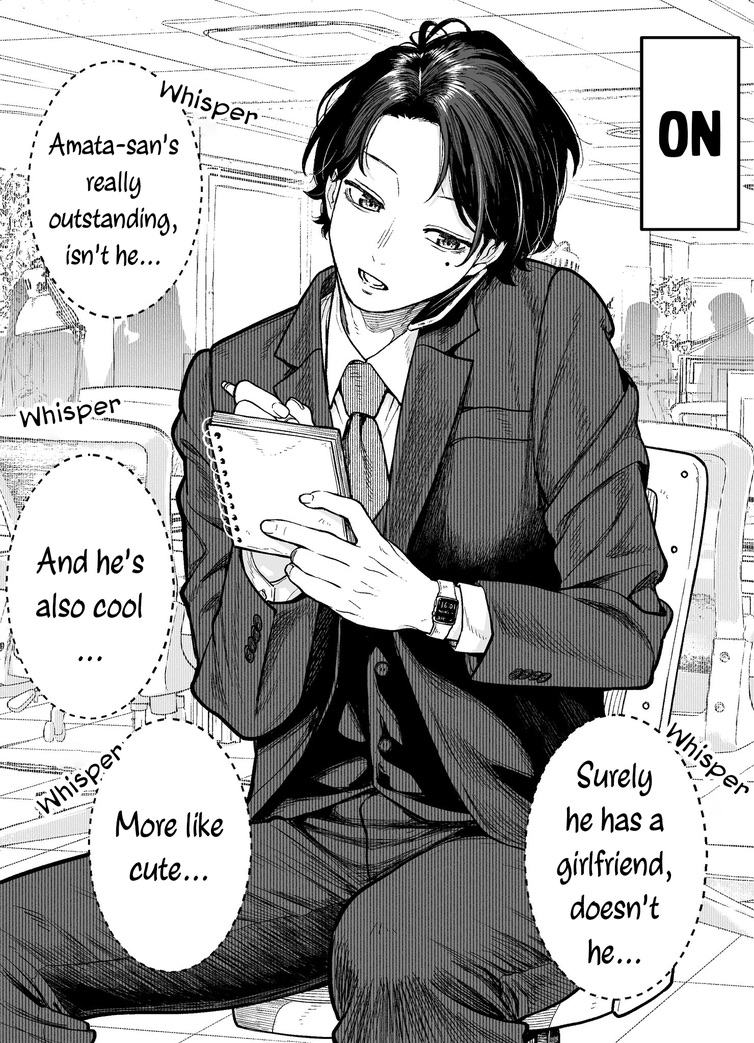
\includegraphics[width=0.4\textwidth]{ch1/on-mode.jpg}
    	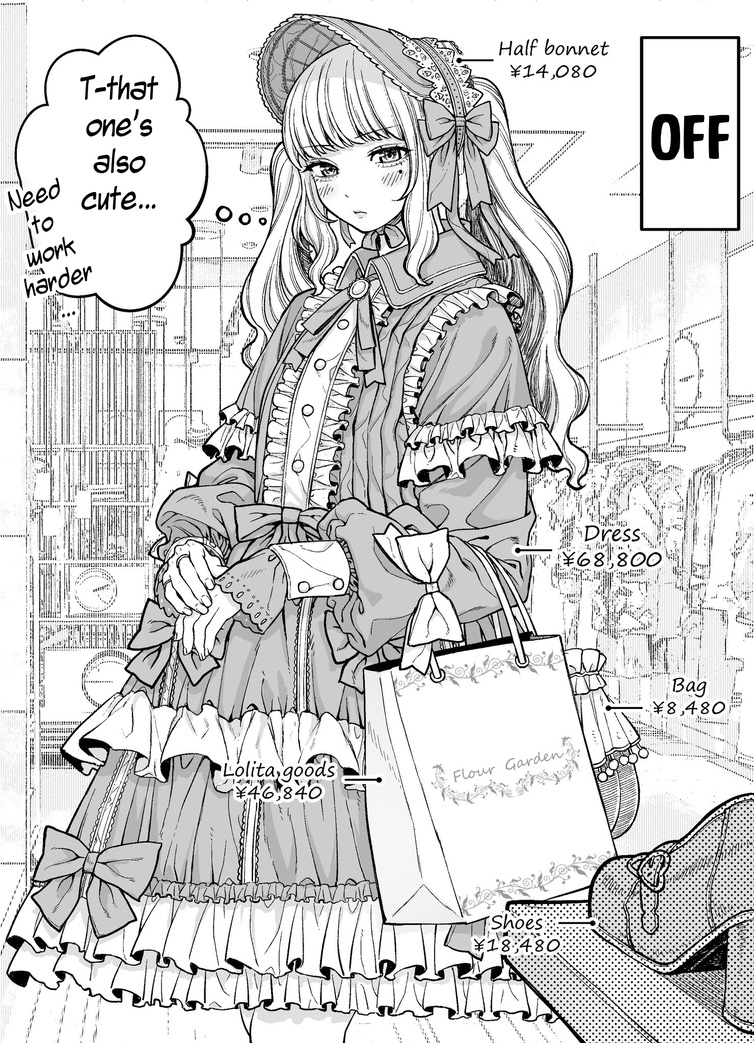
\includegraphics[width=0.4\textwidth]{ch1/off-mode.jpg}
    	\caption{Amata-san's ON and OFF mode. }
    \end{figure}

    \subsection{Another subsection}
    
    \par
    But text only. 
    
\end{spacing}